
\caulc

%%%=============EX_1=============%%%
\begin{ex}%[2D1N2-2]
	Cho bảng biến thiên của hàm số $y=f(x)$ như hình vẽ bên dưới. Giá trị cực tiểu của hàm số là
	\begin{center}
		\begin{tikzpicture}[font=\normalsize,t style/.style={style=solid}]
			\tkzTabInit[nocadre=false, lgt=1.2, espcl=2.5, deltacl=0.5]
			{$x$/0.6,$f(x)$/2}
			{$-\infty$, $1$, $2$, $4$, $+\infty$}
			
			\path
			($(N12)!0.1!(N11)$) node (A1){$-\infty$}
			($(N22)!0.8!(N21)$) node (A2){$ 6 $}
			($(N32)!0.1!(N31)$) node (A3){$ 1 $}
			($(N42)!0.8!(N41)$) node (A4){$ 5 $}
			($(N52)!0.1!(N51)$) node (A5){$ -\infty$};
			
			\foreach \x/\y in {A1/A2, A2/A3, A3/A4, A4/A5}{
				\draw[-stealth] (\x)--(\y);
			}
		\end{tikzpicture}
	\end{center}
	\choice
	{$6$}
	{\True $1$}
	{$5$}
	{$-\infty$}
	\loigiai{
		Theo bảng biến thiên, giá trị cực tiểu của hàm số là $y_{\text{CT}}=1$.
	}
\end{ex}
%%%=============================%%%

%%%=============EX_2=============%%%
\begin{ex}%[1D1N5-3]%[TDMT04]%[Nguyễn Trí Minh Tuấn]
	Nghiệm của phương trình $2\cos x=-\sqrt{3}$ là
	\choice
	{$x=\pm\dfrac{5\pi}{6}+k\pi$, $k\in\mathbb{Z}$}
	{$x=\pm\dfrac{5\pi}{6}+k2\pi$, $k\in\mathbb{N}$}
	{$x=\pm\dfrac{\pi}{6}+k2\pi$, $k\in\mathbb{Z}$}
	{\True $x=\pm\dfrac{5\pi}{6}+k2\pi$, $k\in\mathbb{Z}$}
	\loigiai{
		Ta có $2\cos x=-\sqrt{3} \Leftrightarrow \cos x=-\dfrac{\sqrt{3}}{2} \Leftrightarrow x=\pm\dfrac{5\pi}{6}+k2\pi$, $k\in\mathbb{Z}$
	}
\end{ex}
%%%=============================%%%

%%%=============EX_3=============%%%
\begin{ex}%[2D1N1-2]%[TDMT03]%[Trần Văn Thiện]
	\immini[thm]{Cho đồ thị hàm số $y=f(x)$ như hình vẽ bên. Hàm số đã cho nghịch biến trên khoảng nào dưới đây?
		\choice
		{$\left(-\infty;-1\right)$}
		{$\left(3;+\infty\right)$}
		{\True $\left(-1;3\right)$}
		{$\left(-3;1\right)$}}{
		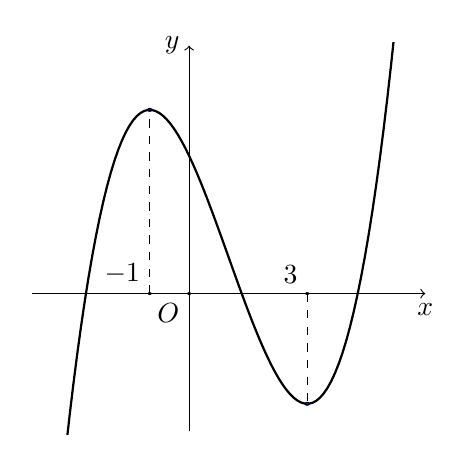
\begin{tikzpicture}[scale=.5,yscale=0.7] 
			\def\xmin{-4};\def\ymin{-5};\def\xmax{6};\def\ymax{9};
			\coordinate (O) at (0,0);
			\draw[->] (\xmin,0)--(\xmax,0) node[below]{$x$};
			\draw[->] (0,\ymin)--(0,\ymax) node[left]{$y$};
			\fill (O) node[below left]{$O$} circle(1.5pt);
			\clip ({\xmin-0.1},{\ymin-0.1}) rectangle ({\xmax+0.1},{\ymax+0.1});
			\foreach \x in {-1,3}{\fill (\x,0) node[above left]{$\x$} circle(1.5pt);}
			\draw[thick,samples=100] plot[domain=\xmin+0.3:\xmax-0.3](\x,{(1/3)*(\x)^3-1*(\x)^2-3*\x+5});
			\draw [fill=blue] (-1,20/3) circle(1.5pt);
			\draw [fill=blue](3,-4) circle(1.5pt);
			\draw[dashed] (-1,0)--(-1,20/3) (3,0)--(3,-4);
		\end{tikzpicture}
	}
	\loigiai{
		Từ đồ thị hàm số ta thấy hàm số $y=f(x)$ nghịch biến trên khoảng $\left(-1;3\right)$.
	}
\end{ex}
%%%=============================%%%

%%%=============EX_4=============%%%
\begin{ex}%[1D6N1-3]%[TDMTD04]%[Phạm Hải Dương]
	Hàm số $y = x^{\pi}$ \textbf{không} cùng tập xác định với hàm số nào dưới đây?
	\choice
	{$y = x^{\mathrm{e}}$}
	{$y = x^{0,7}$}
	{$y = \log x$}
	{\True $y = x^{-2}$}
	\loigiai{Hàm số $y = x^{\pi}$ xác định khi và chỉ khi $x > 0$. Suy ra tập xác định là $\mathscr{D} = (0; +\infty)$.
		\begin{itemize}
			\item Các hàm số $y = x^\mathrm{e}$ (với $\mathrm{e} \notin \mathbb{Z}$), $y = x^{0{,}7}$ (với $0{,}7 \notin \mathbb{Z}$) và $y = \log x$ đều có cùng tập xác định là $(0; +\infty)$.
			\item Hàm số $y = x^{-2}$ xác định khi và chỉ khi $x \neq 0$. Suy ra tập xác định là $\mathscr{D} = \mathbb{R} \setminus \{0\}$.\\
			Vậy hàm số $y = x^{-2}$ không cùng tập xác định với hàm số đã cho.
		\end{itemize}
	}
\end{ex}
%%%=============================%%%

%%%=============EX_5=============%%%
\begin{ex}%[1D2H3-4]%[TDMT03]%[Văn Minh Thoại]
	Cho cấp số nhân $(u_n)$ với $u_1=4$ và công bội $q=\dfrac{1}{2}$. Giá trị của $u_3$ bằng
	\choice
	{$\dfrac{1}{2}$}
	{\True $1$}
	{$2$}
	{$8$}
	\loigiai{
		Ta có công thức số hạng tổng quát của cấp số nhân là $u_n=u_1\cdot q^{n-1}$.\\
		Với $n=3$, ta có
		$u_3=u_1\cdot q^{3-1}=4\cdot\left(\dfrac{1}{2}\right)^2=4\cdot\dfrac{1}{4}=1$.
	}
\end{ex}
%%%=============================%%%

%%%=============EX_6=============%%%
\begin{ex}%[1D6H4-2]%[TDMT04]%[Lê Phúc]
	Tập nghiệm của phương trình $\log_2\left(x^2-1\right)=\log_2(2x-1)$ là
	\choice
	{$\{0;2\}$}
	{\True $\{2\}$}
	{$\varnothing$}
	{$\{0;1;2\}$}
	\loigiai{
		Điều kiện $\heva{&x^2-1>0\\&2x-1>0}\Leftrightarrow \heva{&\hoac{&x<-1\\&x>1}\\&x>\dfrac{1}{2}}\Rightarrow x>1$.\\
		Ta có
		\begin{eqnarray*}
			&&\log_2\left(x^2-1\right)=\log_2(2x-1)\\
			&\Leftrightarrow& x^2-1=2x-1\\
			&\Leftrightarrow& x^2-2x=0\\
			&\Leftrightarrow& \hoac{&x=0\ \text{(không thỏa mãn)}\\&x=2\ \text{(thỏa mãn)}.}
		\end{eqnarray*}
		Vậy tập nghiệm của phương trình là $S=\{2\}$.
	}
\end{ex}
%%%=============================%%%

%%%=============EX_7=============%%%
\begin{ex}%[2D1H5-1]%[TDMT04]%[Vũ Hồng Toàn]
	\immini[thm]{
		Cho một phần đồ thị hàm số $y=\dfrac{ax+2}{x+d}$. Nhận xét đúng về giá trị của các hệ số $a$ và $d$ tương ứng là
		\choice
		{$a<0$, $d<0$}
		{$a>0$, $d>0$}
		{\True $a<0$, $d>0$}
		{$a>0$, $d<0$}
	}
	{
		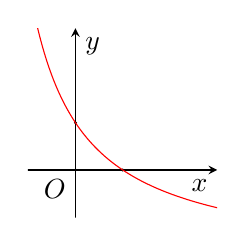
\begin{tikzpicture}[scale=0.6, line join=round, line cap=round,>=stealth]
			\tikzset{declare function={a=-2; b=2; c=1; d=2; f(\x)=(a*(\x)+b)/(c*(\x)+d);
					xmin=-1;xmax=3;	ymin=-1;ymax=3;},
				smooth,samples=200
			}
			\draw[->] (xmin,0)--(0,0) node[below left]{$O$} --(xmax,0) node[below left] {$x$};
			\draw[->] (0,ymin)--(0,ymax) node[below right] {$y$};
			\fill (0,0) circle (1pt);
			\foreach \x/\g in {1/-120} \fill (\x,0) circle (1pt);
			\foreach \y/\g in {1/45} \fill (0,\y) circle (1pt);
			\begin{scope}
				\clip (xmin,ymin) rectangle (xmax,ymax);
				\draw[red,domain=xmin:xmax] plot (\x,{f(\x)});
			\end{scope}
		\end{tikzpicture}
	}
	\loigiai{
		Quan sát đồ thị ta nhận thấy
		\begin{itemize}
			\item Đồ thị của hàm số cắt trục tung tại điểm có tung độ dương nên $\dfrac{2}{d}>0\Rightarrow d>0$.
			\item Đồ thị của hàm số cắt trục hoành tại điểm có hoành độ dương nên $\dfrac{-2}{a}>0\Rightarrow a<0$.
		\end{itemize}
		Vậy giá trị của các hệ số $a$ và $d$ tương ứng là $a<0$, $d>0$.
	}
\end{ex}
%%%=============================%%%

%%%=============EX_8=============%%%
\begin{ex}%[2D1H2-1]%[TDMT04]%[Chu Ha]
	Hàm số $y=x^{3}-12x$ đạt cực đại tại điểm nào sau đây.
	\choice
	{\True $x=-2$}
	{$x=2$}
	{$y=2$}
	{$y=-2$}
	\loigiai{
		\immini{
			Ta có tập xác định là $\mathscr{D}= \mathbb{R}$.\\
			Khi đó $y'=0\Leftrightarrow 3x^2-12 =0\Leftrightarrow
			x=\pm2$.\\
			Lập bảng biến thiên của hàm số như hình bên.\\
			Từ bảng biến thiên, hàm số đồng biến trên $(-\infty;-2)$ và nghịch biến trên $(-2;2)$ nên đạt cực đại tại $x=-2$.
		}
		{
			
\begin{tikzpicture}
				\tkzTabInit[nocadre=false,lgt=1.2,espcl=2]
				{$x$/1,$y'$/1,$y$/2}
				{$-\infty$,$-2$,$2$,$+\infty$}
				\tkzTabLine{,+,0,-,0,+,}
				\tkzTabVar{-/$-\infty$,+/{$y(-2)$},-/{$y(2)$},+/$+\infty$}
			\end{tikzpicture}
		}
	}
\end{ex}
%%%=============================%%%

%%%=============EX_9=============%%%
\begin{ex}%[1H8H7-2]%[TDMT04]%[Nguyễn Sơn Thành]
	\immini[thm]{Cho khối chóp $S.ABC$ có đáy là tam giác vuông cân tại $A$, $AB = 2$, $SA$ vuông góc với đáy và $SA = 3$ (tham khảo hình vẽ bên). Thể tích khối chóp đã cho bằng
		\choice
		{$6$}
		{\True $2$}
		{$3$}
		{$1$}}{\begin{tikzpicture}[declare function={gocx=90; goc=-150; a=3.2; b=a/2; h=3;},scale=.8]
			\path (0,0) coordinate (A)--+(gocx:h) coordinate (S)
			(a,0) coordinate (C)
			(goc:b) coordinate (B);
			\foreach \x/\y/\z in {S/A/C,S/A/B,C/A/B}{
				\path (\y) pic[draw,angle radius=4pt]{right angle = \x--\y--\z};
			}
			\draw[dashed] (S)--(A) (B)--(A)--(C);
			\draw (S)--(B)--(C)--(S)--cycle;
			\foreach \x/\goc in {S/90,A/135,C/-60,B/-180}
			\fill (\x) node[shift={(\goc:7pt)},font=\scriptsize]{$\x$} circle (1pt);
	\end{tikzpicture}}
	\loigiai{ Ta có đáy là tam giác vuông cân tại $A$, diện tích là $S_{ABC} = \dfrac{1}{2} \cdot AB \cdot AC = \dfrac{1}{2} \cdot 2 \cdot 2 = 2$.\\
		Thể tích khối chóp $S. ABC$ là $V_{S. ABC} = \dfrac{1}{3} \cdot S_{ABC} \cdot SA= \dfrac{1}{3} \cdot 2 \cdot 3 = 2$.
	}
\end{ex}
%%%=============================%%%

%%%=============EX_10=============%%%
\begin{ex}%[0D8N2-1]%[Đỗ Đường Hiếu]
	Cho tập $A$ có $10$ phần tử. Số tập con không quá $1$ phần tử của tập $A$ bằng
	\choice
	{$20$}
	{$10$}
	{\True $11$}
	{$2$}
	\loigiai{
		Số tập con không quá $1$ phần tử của $A$ bằng $\mathrm{C}^0_{10}+\mathrm{C}^1_{10}=11$.
	}
\end{ex}
%%%=============================%%%

%%%=============EX_11=============%%%
\begin{ex}%[2D1N3-1]%[TDMT04]%[Huỳnh Quốc Đạt]
	Cho hàm số $f(x)$ có bảng biến thiên như hình vẽ bên dưới. Giá trị lớn nhất của hàm số $f(x)$ trên đoạn $[0;4]$ là
	\begin{center}
		
\begin{tikzpicture}
			\tkzTabInit[nocadre=false,lgt=1.2,espcl=2.5,deltacl=0.6]
			{$x$ /0.6,$f(x)$ /2}
			{$-\infty$,$-4$,$0$,$1$,$+\infty$}
			\tkzTabVar{-/$-\infty$,+/$5$,-/$0$,+/$2$,-/$-\infty$}
		\end{tikzpicture}
	\end{center}
	\choice
	{$1$}
	{$5$}
	{\True $2$}
	{$4$}
	\loigiai{
		Dựa vào bảng biến thiên ta có $\max\limits_{[0;4]}{f(x)}=f(1)=2$.
	}
\end{ex}
%%%=============================%%%

%%%=============EX_12=============%%%
\begin{ex}%[2H2H1-3]%[TDMTD01]%[Dương Công Tạo]
	\immini[thm]{Cho hình lập phương $ABCD.A'B'C'D'$. Hãy tính $\cos\left(\overrightarrow{AB'}, \overrightarrow{BD} \right)$.
		\choice
		{\True $-\dfrac{1}{2}$}
		{$\dfrac{1}{2}$}
		{$-\dfrac{\sqrt{3}}{2}$}
		{$\dfrac{\sqrt{3}}{2}$}}
	{\begin{tikzpicture}
			\def\a{3}
			\path 	(0:0) coordinate (A)
			++(0:\a) coordinate (D)
			++(-130:\a/2) coordinate (C)
			($(A)+(C)-(D)$) coordinate (B)
			($(A)+(90:\a)$) coordinate (A')
			($(B)+(90:\a)$) coordinate (B')
			($(C)+(90:\a)$) coordinate (C')
			($(D)+(90:\a)$) coordinate (D');
			\draw[dashed] 	(B)--(A)--(D)	(A)--(A')	(A)--(B')	(B)--(D);
			\draw	(C)--(C') 	(D)--(D') 	(B)--(B') 	(B)--(C)--(D) (A')--(B')--(C')--(D')--cycle;
			\foreach \x/\g in {A/45,B/180,C/0,D/0,A'/180,B'/180,C'/0,D'/0}
			\fill[black] 	(\x) circle (1pt)
			($(\g:4mm)+(\x)$) node {$\x$};	
		\end{tikzpicture}
	}
	\loigiai{
		Giả sử hình lập phương độ dài cạnh $1$, ta có
		\begin{itemize}
			\item $\left|\overrightarrow{AB'}\right|=\left|\overrightarrow{BD}\right|=\sqrt{2}$.
			\item \begin{eqnarray*}
				\overrightarrow{AB'}\cdot\overrightarrow{BD}&=&\left(\overrightarrow{AA'}+\overrightarrow{AB}\right)\cdot\left(\overrightarrow{AD}-\overrightarrow{AB}\right)\\
				&=&\overrightarrow{AA'}\cdot\overrightarrow{AD}-\overrightarrow{AA'}\cdot\overrightarrow{AB}+\overrightarrow{AB}\cdot\overrightarrow{AD}-\overrightarrow{AB}^2\\
				&=&0-0+0-1^2\\
				&=&-1.
			\end{eqnarray*}
		\end{itemize}
		Khi đó, ta có $\cos\left(\overrightarrow{AB'}, \overrightarrow{BD} \right)=\dfrac{\overrightarrow{AB'}\cdot\overrightarrow{BD}}{\left|\overrightarrow{AB'}\right|\cdot\left|\overrightarrow{BD}\right|}=\dfrac{-1}{\sqrt{2}\cdot\sqrt{2}}=-\dfrac{1}{2}$.
		
	}
\end{ex}
%%%=============================%%%

\cauds

%%%=============EX_13=============%%%
\begin{ex}%[2D1H3-2]%[TDMT04]%[Nguyễn Tấn Linh]
	Cho hàm số $f(x) = \mathrm{e}^x - x + 4$. Hỏi mệnh đề nào dưới đây là đúng hay sai?
	\choiceTF
	{\True Tập xác định của hàm số là $\mathscr{D} = \mathbb{R}$}
	{\True $f'(x) = \mathrm{e}^x - 1$}
	{\True $f'(x) = 0 \Leftrightarrow x = 0$}
	{\True $\min\limits_{x\in\mathscr{D}} f(x) = 5$}
	\loigiai{
		\begin{itemchoice}
			\itemch Tập xác định của hàm số là $\mathscr{D} = \mathbb{R}$.
			\itemch Ta có $f'(x) = \mathrm{e}^x - 1$.
			\itemch Ta có $f'(x) = 0 \Leftrightarrow \mathrm{e}^x - 1 = 0 \Leftrightarrow x = 0$.
			\itemch Kẻ bảng biến thiên
			\begin{center}
				
\begin{tikzpicture}[>=stealth]
					\tkzTabInit[nocadre=false,lgt=1.2,espcl=2.5,deltacl=0.6]
					{$x$ /1,$f'(x)$ /1,$f(x)$ /1.5}
					{$-\infty$, $0$, $+\infty$}
					\tkzTabLine{ ,-,0,+, }
					\tkzTabVar{+/ $+\infty$,-/ $5$, +/ $+\infty$}
				\end{tikzpicture}
			\end{center}
			Dựa vào bảng biến thiên ta có $\min\limits_{x\in\mathscr{D}} f(x) = 5$.
		\end{itemchoice}
	}
\end{ex}
%%%=============================%%%

%%%=============EX_14=============%%%
\begin{ex}%[Duong Xuan Loi]%[1H8V7-8]
	Cho hình lăng trụ đều $ABC. A'B'C'$ có cạnh đáy bằng $4$ và chiều cao bằng $6$.
	\choiceTF
	{\True Thể tích của lăng trụ $ABC. A'B'C'$ bằng $24\sqrt{3}$}
	{\True Thể tích của hình chóp $A. A'B'C'$ bằng $8\sqrt{3}$}
	{\True $\mathrm{d}\left(A', (AB'C')\right) = 3$}
	{Góc tạo bởi hai đường thẳng $AB'$, $BC'$ tính theo đơn vị độ bằng $63^\circ$ \textit{ (làm tròn kết quả đến hàng đơn vị)}}
	\loigiai{
		\begin{center}
			\begin{tikzpicture}[scale=0.8, line join=round, line cap=round, >=stealth]
				\coordinate (A') at (0,0);
				\coordinate (B') at (4,0);
				\coordinate (C') at (1.5,1.5);
				\coordinate (A) at (0,5);
				\coordinate (B) at (4,5);
				\coordinate (C) at (1.5,6.5);
				\coordinate (M) at ($(B')!0.5!(C')$);
				\coordinate (D') at ($(A')+(C')-(B')$); 				
				\draw (A)--(B)--(C)--(A) (A)--(A')--(D') (B)--(B') (B')--(A') (A)--(B') ;
				\draw[dashed] (C)--(C') (C')--(A') (C')--(B') (A)--(M) (A')--(M) (A)--(C')--(B);
				\draw[dashed] (D') -- (C'); 
				\draw (A) -- (D');				
				\foreach \p/\pos in {A/left, B/right, C/above, A'/below, B'/below, C'/below, D'/left, M/below}
				\fill (\p) circle (1.0pt) node[\pos] {$\p$};
			\end{tikzpicture}
		\end{center}
		\begin{itemchoice}
			\itemch Diện tích đáy tam giác đều $ABC$ là $S_{\triangle ABC} = \dfrac{4^2\sqrt{3}}{4} = 4\sqrt{3}$.\\
			Thể tích khối lăng trụ $V_{ABC. A'B'C'} = S_{\triangle ABC} \cdot AA' = 4\sqrt{3} \cdot 6 = 24\sqrt{3}$.
			\itemch Khối chóp $A. A'B'C'$ có diện tích đáy $S_{\triangle A'B'C'} = S_{\triangle ABC} = 4\sqrt{3}$ và chiều cao $AA' = 6$.\\
			Thể tích khối chóp: $V_{A. A'B'C'} = \dfrac{1}{3} S_{\triangle A'B'C'} \cdot AA' = \dfrac{1}{3} \cdot 24\sqrt{3} = 8\sqrt{3}$.
			\itemch Gọi $h = \mathrm{d}(A', (AB'C'))$.\\ Xét khối chóp $A'. AB'C'$ có $V_{A'. AB'C'} = V_{A. A'B'C'} = 8\sqrt{3}$.\\
			Tam giác $AB'C'$ cân tại $A$ có $B'C' = 4$, $AB'=AC'=\sqrt{6^2+4^2}=2\sqrt{13}$.\\
			Đường cao $AM=\sqrt{AB'^2-\left(\dfrac{B'C'}{2}\right)^2}=\sqrt{52-4}=4\sqrt{3}$.\\
			Diện tích $S_{\triangle AB'C'} = \dfrac{1}{2} \cdot 4 \cdot 4\sqrt{3} = 8\sqrt{3}$.\\
			Vậy $h = \dfrac{3 \cdot V_{A'. AB'C'}}{S_{\triangle AB'C'}} = \dfrac{3 \cdot 8\sqrt{3}}{8\sqrt{3}} = 3$.
			\itemch Lấy điểm $D'$ sao cho $A'B'C'D'$ là hình bình hành.\\
			Suy ra $C'D'\parallel A'B'$, $C'D' = A'B' = 4$, mà $A'B'\parallel AB$ và $A'B' = AB=4$.\\
			Do đó $ABC'D'$ là hình bình hành $\Rightarrow BC' \parallel AD'$. \\
			Khi đó $(AB', BC') = (AB', AD')$.\\
			Xét $\triangle AB'D'$ có $AD' = AB' = 2\sqrt{13}$.
			\[B'D' = \sqrt{A'B'^2+A'D'^2-2A'B'\cdot A'D' \cdot \cos 120^\circ} = \sqrt{4^2 + 4^2 - 2 \cdot 4 \cdot 4 \cdot \left(-\dfrac{1}{2}\right)} = 4\sqrt{3}.\]
			Áp dụng định lý hàm số côsin trong $\triangle AB'D'$: \\
			$\cos \widehat{B'AD'} = \dfrac{AB'^2 + AD'^2 - B'D'^2}{2 \cdot AB' \cdot AD'} = \dfrac{52 + 52 - 48}{2 \cdot 52} = \dfrac{56}{104} = \dfrac{7}{13}$.\\
			Vậy $\widehat{B'AD'} \approx 57^\circ \neq 63^\circ$.
		\end{itemchoice}
	}
\end{ex}
%%%=============================%%%

%%%=============EX_15=============%%%
\begin{ex}%[0D8V2-7]
	Gọi $S$ là tập gồm tất cả các chuỗi dài $8$ kí tự, chỉ gồm có hai loại kí tự A và B. Ví dụ: AABABBAB, BBABBAAB. Hỏi trong các mệnh đề dưới đây, mệnh đề nào đúng, mệnh đề nào sai ?
	\choiceTF
	{\True Số phần tử của $S$ là $256$}
	{\True Số phần tử của $S$ mà chỉ có đúng một loại kí tự A hoặc B là $2$}
	{\True Số phần tử của $S$ sao cho số kí tự A bằng số kí tự B là $70$}
	{\True Số phần tử của tập $S$ sao cho không có hai kí thự B nào đứng cạnh nhau (ví dụ như là: AAABABAA) là $55$}
	\loigiai{
		\begin{itemchoice}
			\itemch Với $8$ vị trí, mỗi vị trí có $2$ cách chọn, tổng số chuỗi là: $2 \times 2 \times 2 \times 2 \times 2 \times 2 \times 2 \times 2 = 2^8 = 256$.
			\itemch Chuỗi toàn ký tự A: AAAAAAAA;
			Chuỗi toàn ký tự B: BBBBBBBB.
			\itemch Chuỗi dài $8$ ký tự, số ký tự A bằng số ký tự B thì mỗi loại phải có đúng $4$ ký tự.\\
			Chọn $4$ vị trí trong $8$ vị trí để đặt ký tự A ($4$ vị trí còn lại tự động là B) có $\mathrm{C}_8^4 =70$.
			\itemch Chia các trường hợp:\\
			\textbf{Trường hợp 1.} Chuỗi không có chữ B nào (toàn A) nên có $1$ chuỗi: AAAAAAAA.\\
			\textbf{Trường hợp 2.} Chuỗi có $1$ chữ B. Chữ B có thể đứng ở bất kỳ vị trí nào trong $8$ vị trí có $8$ chuỗi.\\
			\textbf{Trường hợp 3.} Có $2$ chữ B.\\
			Đặt $6$ chữ A tạo ra $7$ khoảng trống ($5$ khe giữa và $2$ đầu): - A - A - A - A - A - A -\\
			Chọn $2$ khoảng trống trong $7$ để đặt B: $\mathrm{C}_7^2 = 21$ cách.\\
			\textbf{Trường hợp 4.} Có $3$ chữ B.\\
			Đặt $5$ chữ A tạo ra $6$ khoảng trống: - A - A - A - A - A -.\\
			Chọn $3$ khoảng trống trong $6$ để đặt B: $\mathrm{C}_6^3 = 20$ cách.\\
			\textbf{Trường hợp 5.} Có $4$ chữ B.\\
			Đặt $4$ chữ A tạo ra $5$ khoảng trống: - A - A - A - A -\\
			Chọn $4$ khoảng trống trong $5$ để đặt B: $\mathrm{C}_5^4 = 5$ cách.\\
			Tổng số chuỗi thỏa mãn là: $1 + 8 + 21 + 20 + 5 = 55$.
		\end{itemchoice}
	}
\end{ex}
%%%=============================%%%

%%%=============EX_16=============%%%
\begin{ex}%[2D1V5-7]%[TDMT04]%[Lê Hồ Quang Minh]
	Cho hàm số $y = f(x) = \dfrac{x^2 - 3x + 2}{x - 3}$ có đồ thị $(C)$.
	\choiceTF
	{\True $(C)$ có tiệm cận đứng là $x = 3$ và tiệm cận xiên là $y = x$}
	{$(C)$ có đường thẳng đi qua hai điểm cực trị là $y = x - 3$}
	{Hàm số $\dfrac{f(x)}{x - 1}$ nghịch biến trên các khoảng $(-\infty; 3)$, $(3; +\infty)$}
	{\True Có tất cả $10$ đường thẳng (không song song với $Oy$) có điểm chung với $(C)$, các điểm chung này đều có tọa độ nguyên}
	\loigiai{
		Xét hàm số $f(x) = \dfrac{x^2 - 3x + 2}{x - 3}$.\\ Tập xác định $\mathscr{D}= \mathbb{R} \setminus \{3\}$.
		\begin{itemchoice}
			\itemch Ta có $f(x) = x + \dfrac{2}{x-3}$.
			\begin{itemize}
				\item $\displaystyle\lim\limits_{x \to 3} f(x) = \infty \Rightarrow x = 3$ là tiệm cận đứng.
				\item $\displaystyle\lim\limits_{x \to \infty} [f(x) - x] = \displaystyle\lim\limits_{x \to \infty} \dfrac{2}{x-3} = 0 \Rightarrow y = x$ là tiệm cận xiên.
			\end{itemize}
			\itemch Đường thẳng đi qua hai điểm cực trị có phương trình $y = \dfrac{\left(x^2-3x+2\right)'}{\left(x-3\right)'} = 2x - 3$.
			\itemch Hàm số $g(x) = \dfrac{f(x)}{x-1} = \dfrac{x^2 - 3x + 2}{(x-3)\cdot(x-1)}$ có tập xác định $\mathscr{D}= \mathbb{R} \setminus \{1;3\}$.\\
			Khi đó $g(x) = \dfrac{x-2}{x-3}$.\\
			Suy ra $g'(x) = \dfrac{-1}{(x-3)^2} < 0$, $\forall x \in \mathscr{D}$.\\ 
			Vậy hàm số nghịch biến trên các khoảng $\left(-\infty;1\right)$, $\left(1;3\right)$ và $\left(3;+\infty\right)$.\\ Mệnh đề sai vì hàm số gián đoạn tại $x=1$.
			\itemch 
			\begin{itemize}
			\item \textbf{Cách 1:} Gọi $M(x_0; y_0) \in (C)$ là điểm có tọa độ nguyên.\\
			Suy ra $y_0 = x_0 + \dfrac{2}{x_0-3}$.\\
			Vì $x_0$, $y_0 \in \mathbb{Z}$ nên $(x_0-3)$ là ước của $2$.\\
			Ta có $x_0-3 \in \{\pm 1; \pm 2\} \Rightarrow x_0 \in \{2; 4; 1; 5\}$.\\
			Khi đó có $4$ điểm có tọa độ nguyên là $M_1(2; 0)$, $M_2(4; 6)$, $M_3(1; 0)$, $M_4(5; 6)$.\\
			Mỗi cách chọn $2$ trong $4$ điểm trên là một tổ hợp chập $2$ của $4$.\\
			Suy ra có $\mathrm{C}_4^2 = 6$ đường thẳng đi qua $2$ trong $4$ điểm trên (đều có điểm chung nguyên).\\
			Ngoài ra, tại mỗi điểm $M_i$ nói trên, ta kẻ được $1$ tiếp tuyến với đồ thị (các tiếp tuyến này không song song với $Oy$).\\ Điểm chung của tiếp tuyến và $(C)$ chính là tiếp điểm có tọa độ nguyên.\\
			Suy ra có thêm $4$ đường thẳng là tiếp tuyến tại $4$ điểm này.\\
			Vậy có tất cả $6 + 4 = 10$ đường thẳng thỏa mãn (lưu ý kiểm tra lại các đường thẳng này đều không song song với $Oy$).
			\item \textbf{Cách 2:} Gọi $(d)\colon y = ax+b$ ($a\neq 0$) là đường thẳng thỏa mãn yêu cầu.\\
			Phương trình hoành độ giao điểm của $(d)$ và $(C)$:
			\[ax+b = x + \dfrac{2}{x-3} \Leftrightarrow (a-1)x + b = \dfrac{2}{x-3}.\]
			Để giao điểm có tọa độ nguyên thì $x$ nguyên và $\dfrac{2}{x-3}$ nguyên.\\ Suy ra $(x-3) \in \text{Ư}(2) = \{\pm 1; \pm 2\}$.\\
			Từ đó ta tìm được đúng $4$ điểm nguyên trên đồ thị $(C)$ là $M_1$, $M_2$, $M_3$, $M_4$ như trên.\\
			Đường thẳng cần tìm sẽ là các đường thẳng nối $2$ điểm bất kỳ trong $4$ điểm này hoặc là các tiếp tuyến tại $4$ điểm này.\\
			Tổng số đường thẳng là $\mathrm{C}_4^2 + 4 = 6+4=10$.
			\end{itemize}
		\end{itemchoice}
	}
\end{ex}
%%%=============================%%%

\caukq

%%%=============EX_17=============%%%
\begin{ex}%[1H8V7-3]%[TDMT04]%[Lương Pho]
	Cho hình chóp tứ giác đều $S. ABCD$ có chiều cao, độ dài cạnh đáy, độ dài cạnh bên theo thứ tự lập thành một cấp số cộng có công sai bằng $2$. Hãy tính thể tích của $S. ABCD$ (\textit{làm tròn kết quả đến hàng đơn vị})?
	\par
	\shortans[0]{1195}
	\loigiai{
		\immini{
			Gọi $h$ là chiều cao, $a$ là độ dài cạnh đáy và $b$ là độ dài cạnh bên của hình chóp tứ giác đều $S. ABCD$.\\
			Theo đề bài $h$, $a$, $b$ lập thành cấp số cộng có công sai bằng $2$ nên
			\[\heva{&a = h + 2 \\ &b = h + 4}\text{ (với $h > 0$).}\]
			Gọi $O$ là tâm của đáy $ABCD$, suy ra $SO \perp (ABCD)$ và $SO = h$.\\
			Trong tam giác vuông $SOC$, ta có
			\begin{eqnarray*}
				SC^2=SO^2+OC^2 &\Leftrightarrow & b^2 = h^2 + \left(\dfrac{a\sqrt{2}}{2}\right)^2\\
				&\Leftrightarrow & (h+4)^2=h^2+\left[\dfrac{(h+2)\sqrt{2}}{2}\right]^2\\
				&\Leftrightarrow & 2(h+4)^2=2h^2+(h+2)^2\\
				&\Leftrightarrow & -h^2+12h+28 = 0\\
				&\Leftrightarrow & \hoac{&h=14 \text{ (nhận)}\\&h=-2\text{ (loại).}}
		\end{eqnarray*}}{
			\begin{tikzpicture}[font=\footnotesize, scale=1, line join =round, line cap= round, >= stealth,
				declare function={goc=-140; a=4; b=0.65*a; h=3.5;gocnghieng=80;}]
				\path 
				(0,0) coordinate (A)
				(a,0) coordinate (D)
				(goc:b) coordinate (B)
				($(D)+(B)-(A)$) coordinate (C)
				($(A)!.5!(C)$) coordinate (O)
				($(O)+(90:h)$) coordinate (S)
				;
				\draw (S)--(C)--(D)--(S)--(B)node[midway,left]{$b$}--(C)node[midway,below]{$a$}
				pic[draw, angle radius=2mm]{right angle =S--O--C};
				\draw[dashed](S)--(A)--(B)  (A) -- (D) (A)--(C)(B)--(D) (S)--(O)node[midway,left]{$h$};
				\foreach \x/\g in {S/150,A/160, B/-120, C/-30,D/0,O/-90} {
					\fill (\x) node[shift={(\g:7pt)}]{$\x$} circle (1pt);
				}
			\end{tikzpicture}
		}
		\noindent Với $h = 14 \Rightarrow a = h+2=16$.\\
		Thể tích khối chóp $S. ABCD$ là
		\[V = \dfrac{1}{3} \cdot S_{ABCD} \cdot SO = \dfrac{1}{3} \cdot 16^2 \cdot 14 = \dfrac{3\,584}{3} \approx 1\,195.\]
	}
\end{ex}
%%%=============================%%%

%%%=============EX_18=============%%%
\begin{ex}%[2D1V5-8]%[TDMT04]%[Võ Hiệp]
	Trong $20$ phút theo dõi, lưu lượng nước của một con sông được tính theo công thức $Q(t)=-200t^3+5\,000t^2+100\,000$, trong đó $Q$ tính theo đơn vị kg/phút, $t$ tính theo phút ($0 \leq t \leq 20$). Khi lưu lượng nước của con sông lên đến $550\,000$ kg/phút thì đưa ra cảnh báo lũ và bắt đầu thấp hơn thì thông báo an toàn. Xác định theo phút khoảng thời gian tồn tại cảnh báo lũ \textit{(làm tròn kết quả đến hàng phần trăm)}?
	\par
	\shortans[0]{3{,}23}
	\loigiai{
		Xét hàm số lưu lượng nước trên đoạn $[0; 20]$:
		$Q(t) = -200t^3 + 5\,000t^2 + 100\,000$.\\
		Khi lưu lượng nước của con sông ở mức $550\,000$ kg/phút thì
		\begin{eqnarray*}
			Q(t) &=& -200t^3 + 5\,000t^2 + 100\,000=550\,000\\
			&\Leftrightarrow&
			-200t^3 + 5\,000t^2 - 450\,000=0\Leftrightarrow
			\hoac{&t=15\in[0; 20]\\&t=5+5\sqrt{7}\in[0; 20].}\\
		\end{eqnarray*}
		Đạo hàm $Q'(t) = -600t^2 + 10\,000t$.\\
		Cho $Q'(t) = 0\Leftrightarrow -600t^2 + 10\,000t = 0 \Leftrightarrow
		\hoac{&t = 0 \\& t = \dfrac{50}{3}.}$\\
		Bảng biến thiên
		\begin{center}
			\begin{tikzpicture}[ >=stealth]
				\tkzTabInit[nocadre=false,lgt=1.2,espcl=2.5,deltacl=1.5]
				{$t$ /0.8,$Q'(t)$ /0.8,$Q(t)$ /2.7}
				{$0$,$15$,$\tfrac{50}{3}$,$5+5\sqrt{7}$,$20$}
				\tkzTabLine{, ,+,, 0,, -,}
				\path(T13)+(30:0.7) node (1) {$Q(0)$};
				\path ($(N22)!.5!(N23)$) node (2) {$550\,000$};
				\path(N32)+(-90:0.5) node (3) {$Q\left(\tfrac{50}{3}\right)$};
				\path ($(N42)!.5!(N43)$) node (4) {$550\,000$};
				\path(T23)+(150:0.7) node (5) {$Q\left(20\right)$};
				\draw[->] (1)--(2);
				\draw[->] (2)--(3);
				\draw[->] (3)--(4);
				\draw[->] (4)--(5);
				\draw[thin,dotted] (N21)--(2) (N41)--(4);
			\end{tikzpicture}
		\end{center}
		Dựa vào bảng biến thiên, ta thấy lưu lượng nước của con sông lên đến $550\,000$ kg/phút tại thời điểm $t=15$ phút và tiếp tục tăng đến đỉnh lũ tại thời điểm $t=\dfrac{50}{3}$ phút. Sau đó lưu lượng nước của con sông giảm xuống $550\,000$ kg/phút tại thời điểm $t=5+5\sqrt{7}$ phút.\\
		Do đó khoảng thời gian tồn tại cảnh báo lũ là $5+5\sqrt{7}-15 \approx 3{,}23$ phút.
		
	}
\end{ex}
%%%=============================%%%

%%%=============EX_19=============%%%
\begin{ex}%[0D8V1-2]%[TDMT02]%[Nguyễn Đức Tuấn Anh]
	\immini[thm]{
		Một hồ thả cá cảnh có dạng hình tổ ong (minh hoạ như hình bên) được thiết kế ở một khu vườn sinh thái. Hồ cá được bao xung quanh bởi $120$ viên đá hình lục giác đều bằng nhau, các viên đá được xếp sao cho các cạnh tiếp xúc là trùng nhau, mỗi viên đá có độ dài một cạnh bằng $20$ cm. Hãy tính diện tích của hồ cá (không tính đường bao quanh) theo đơn vị mét vuông (\textit{làm tròn kết quả đến hàng đơn vị})?}{
		\begin{tikzpicture}[line join=round, line cap=round, >=stealth, scale=1]
			\def \goc{60} \def \r{0.3} \pgfmathsetmacro{\a}{\r*sqrt(3)}
			\tikzset{lucgiac/.pic={
					\path
					(\goc:\r) coordinate (A)
					({2*\goc}:\r) coordinate (B)
					({3*\goc}:\r) coordinate (C)
					({4*\goc}:\r) coordinate (D)
					({5*\goc}:\r) coordinate (E)
					({6*\goc}:\r) coordinate (F);
					\draw[top color=gray!10, bottom color=gray!80, draw=black] (A)--(B)--(C)--(D)--(E)--(F)--cycle;	
			}}
			\tikzset{lucgiacnetdut/.pic={
					\path
					(\goc:\r) coordinate (A)
					({2*\goc}:\r) coordinate (B)
					({3*\goc}:\r) coordinate (C)
					({4*\goc}:\r) coordinate (D)
					({5*\goc}:\r) coordinate (E)
					({6*\goc}:\r) coordinate (F);
					\draw[dashed] (A)--(B)--(C)--(D)--(E)--(F)--cycle;	
			}}
			\foreach \n [count=\i] in {0,1,...,5}{
				\path ($(0:0)+(-30:\n*\a)$) coordinate (M\i);}
			\foreach \n [count=\i from 7] in {1,...,5}{
				\path ($(M6)+(-90:\n*\a)$) coordinate (M\i);}
			\foreach \n [count=\i from 12] in {1,...,5}{
				\path ($(M11)+(-150:\n*\a)$) coordinate (M\i);}
			\foreach \a in {1,2,5,6,7,10,11,12,15,16}{\path (M\a)pic{lucgiac};}
			\path ($(M3)!.5!(M4)$)pic{lucgiacnetdut}
			($(M8)!.5!(M9)$)pic{lucgiacnetdut}
			($(M13)!.5!(M14)$)pic{lucgiacnetdut};
			\begin{scope}[rotate=180, transform shape,shift={(90:17.345*\r)}]
				\foreach \n [count=\i] in {0,1,...,5}{
					\path ($(0:0)+(-30:\n*\a)$) coordinate (M\i);}
				\foreach \n [count=\i from 7] in {1,...,5}{
					\path ($(M6)+(-90:\n*\a)$) coordinate (M\i);}
				\foreach \n [count=\i from 12] in {1,...,5}{
					\path ($(M11)+(-150:\n*\a)$) coordinate (M\i);}
				\foreach \a in {1,2,5,6,7,10,11,12,15,16}{\path (M\a)pic{lucgiac};}
				\path ($(M3)!.5!(M4)$)pic{lucgiacnetdut}
				($(M8)!.5!(M9)$)pic{lucgiacnetdut}
				($(M13)!.5!(M14)$)pic{lucgiacnetdut};
			\end{scope}
		\end{tikzpicture}
	}
	\par 
	\shortans[oly]{119}
	\loigiai{
		\begin{center}
			\begin{tikzpicture}[line join=round, line cap=round, >=stealth, scale=1]
				\def \goc{60} \def \r{0.3} \pgfmathsetmacro{\a}{\r*sqrt(3)}
				\tikzset{lucgiac/.pic={
						\path
						(\goc:\r) coordinate (A)
						({2*\goc}:\r) coordinate (B)
						({3*\goc}:\r) coordinate (C)
						({4*\goc}:\r) coordinate (D)
						({5*\goc}:\r) coordinate (E)
						({6*\goc}:\r) coordinate (F);
						\draw[top color=gray!10, bottom color=gray!80, draw=black] (A)--(B)--(C)--(D)--(E)--(F)--cycle;	
				}}
				\path (0,0) pic{lucgiac};
				\begin{scope}[shift={(0:2)}]
					% Tầng 1
					\foreach \n [count=\i] in {1,2,...,6}{
						\path (\n*60+30:\a)coordinate (M\i);}
					\foreach \a in {1,2,...,6}{\path (M\a)pic{lucgiac};}
					\path (0,-2) node{$1+6$ hình lục giác};
				\end{scope}
				\begin{scope}[shift={(0:6)}]
					% Tầng 2
					\foreach \n [count=\i] in {1,2,...,6}{
						\path (\n*60+30:2*\a)coordinate (M\i);
						\path ($(M\i)+(\n*60-90:\a)$)coordinate (N\i);}
					\foreach \a in {1,2,...,6}{\path (M\a)pic{lucgiac} (N\a)pic{lucgiac};}
					\path (0,-2) node{$1+6+12$ hình lục giác};
				\end{scope}
				\begin{scope}[shift={(0:11)}]
					% Tầng 3
					\foreach \n [count=\i] in {1,2,...,6}{
						\path (\n*60+30:3*\a)coordinate (M\i);
						\path ($(M\i)+(\n*60-90:\a)$)coordinate (N\i);
						\path ($(N\i)+(\n*60-90:\a)$)coordinate (P\i);}
					\foreach \a in {1,2,...,6}{\path (M\a)pic{lucgiac} (N\a)pic{lucgiac} (P\a)pic{lucgiac};}
					\path (0,-2) node{$1+6+12+18$ hình lục giác};
				\end{scope}
				\path (15,-2) node{......};
			\end{tikzpicture}
		\end{center}
		Vì các viên đá xếp sát nhau tạo thành vòng khép kín quanh hồ, nên số lượng đá ở vòng ngoài cùng tuân theo quy luật của lưới lục giác đều.\\
		Số lục giác ở vòng thứ $n$ là $6n$.\\
		Theo bài ra, vòng đá bao quanh có $120$ viên, ta có phương trình $6n = 120 \Rightarrow n = 20$.\\
		Vậy vòng đá bao quanh là vòng thứ $20$.\\ Diện tích mặt hồ (phần bên trong) chính là tổng diện tích của các viên lục giác từ tâm (coi là vòng $0$) đến vòng thứ $19$.\\
		Tổng số viên lục giác tạo thành mặt hồ là
		\[N = 1 + \sum_{k=1}^{19} 6k = 1 + 6 \cdot \dfrac{19\cdot(19+1)}{2} = 1 + 6 \cdot 190 = 1\,141 \text{ (viên)}.\]
		Ta có $a = 20\,(\text{cm}) = 0{,}2\,(\text{m})$.\\
		Diện tích một viên đá lục giác đều là
		\[S_1 = 6 \cdot \dfrac{a^2\sqrt{3}}{4} = \dfrac{3\sqrt{3}}{2} \cdot (0{,}2)^2 = 0{,}06\sqrt{3}\,\left(\text{m}^2\right).\]
		Diện tích của hồ cá là
		\[S = N \cdot S_1 = 1\,141 \cdot 0{,}06\sqrt{3} \approx 118{,}58 \approx 119 \,\left(\text{m}^2\right).\]
	}
\end{ex}
%%%=============================%%%

%%%=============EX_20=============%%%
\begin{ex}%%[0H9V4-7]%[TDMT04]%[Bồ Văn Hậu]
	\immini[thm]{Hai mô đất nhỏ $I$ và $II$ coi như hai hình tròn cùng bán kính bằng $5$ mét, có khoảng cách từ một điểm thuộc hai mô đất này đến bờ gần nhất lần lượt là $15$ mét và $35$ mét. Biết khoảng cách gần nhất giữa hai điểm thuộc hai mô đất là $10\left(\sqrt{13}-1\right)$ mét. Người ta nối một đường dây từ điểm $A$ thuộc mô đất $I$ đến gặp bờ tại điểm $C$, rồi từ $C$ nối với điểm $B$ thuộc mô đất $II$. Hãy tính giá trị nhỏ nhất của tổng quãng đường $AC + CB$ theo đơn vị mét (\textit{làm tròn kết quả đến hàng phần mười}).}{\begin{tikzpicture}[>=stealth, scale=0.1]
			\draw[red, thick] (-15,0) -- (55,0) node[above left, black] {Bờ};
			\coordinate (O1) at (0,20);
			\coordinate (O2) at (30,40);
			\coordinate (C) at (10,0);
			\coordinate (A) at (2.23,15.53);
			\coordinate (B) at (27.77,35.53);
			\draw[blue, thick, fill=green!20] (O1) circle (5);
			\node at (0,20) {\textbf{\textit{I}}};
			\draw[red, thick, fill=cyan!15] (O2) circle (5);
			\node at (30,40) {\textbf{\textit{II}}};
			\draw[thick] (A) -- (C) -- (B);
			\fill (A) circle (0.5) node[below left] {$A$};
			\fill (B) circle (0.5) node[below right] {$B$};
			\fill (C) circle (0.5) node[below] {$C$};
	\end{tikzpicture}}
	\par 
	\shortans[0]{57{,}1}
	\loigiai{
		\immini{Gọi $L$, $E$ lần lượt là tâm của mô đất $I$, $II$.\\
			Chọn hệ trục tọa độ $Oxy$ như hình vẽ bên.\\
			Khi đó $L(0;20)$; $E(x_0;40)$, với $x_0>0$.\\
			Gọi $H(x_0;20)$ là hình chiếu vuông góc của $L$ lên $EK$, với $K(x_0;0)$.\\
			Lấy điểm $M$ trên mô đất $I$ và $N$ trên mô đất $II$.\\
			Ta có $MN\geq LE - 5-5$ hay $MN$ nhỏ nhất là $LE-10$.\\
			Suy ra $LE=10\sqrt{13}$ (mét).\\
			Mà $LE\,^2=LH^2+EH^2$ nên $1\,300=x_0^2+(40-20)^2 \Leftrightarrow x_0^2=900$ hay $x_0=30$ (vì $x_0>0$).\\
			Gọi hình tròn $III$ có tâm $J$, bán kính bằng $5$ đối xứng với hình tròn $I$ qua trục $Ox$ và điểm $D$ đối xứng với $A$ qua trục $Ox$, khi đó $J(0,-20)$.\\
			Ta có $Ox$ là đường trung trực của $AD$ nên $AC=DC$.\\
			Suy ra $AC+CB=DC+CB\geq EJ-10$.\\
			Dấu đẳng thức xảy ra khi $C$ là giao điểm của $EJ$ với trục $Ox$ và $D$, $B$ lần lượt là giao điểm của $EJ$ với hình tròn $III$, $I$.\\
			Mà $\overrightarrow{EJ}=(-30;-60)$ nên $EJ=\sqrt{900+3\,600}=30\sqrt{5}$.\\
			Vậy giá trị nhỏ nhất của tổng quãng đường $AC + CB$ là \[EJ-10=30\sqrt{5}-10\approx 57{,}1 \, \text{(mét)}.\] }{\begin{tikzpicture}[font=\footnotesize,>=stealth, scale=0.12]
				\draw[red, thick, ->] (-10,0) -- (35,0) node[above, black] {$x$} node[below, black] {Bờ};
				\draw[red, thick, ->] (0,-30) -- (0,50) node[right, black] {$y$};
				\coordinate (O) at (0,0);
				\coordinate (L) at (0,20);
				\coordinate (J) at (0,-20);
				\coordinate (E) at (30,40);
				\coordinate (K) at (30,0);
				\coordinate (H) at (30,20);
				\coordinate (C) at (10,0);
				\coordinate (A) at (2.23,15.53);
				\coordinate (D) at (2.23,-15.53);
				\coordinate (B) at (27.77,35.53);
				\draw[red, dashed] (E) -- (0,40) node[left] {$40$};
				\node[red, below left] at (L) {$20$};
				\draw[blue, thick] (L) circle (5);
				\draw[blue, thick] (J) circle (5);
				\draw[red, thick] (E) circle (5);
				\draw[thick] (L)--(A) -- (C) -- (B)--(E) (J)--(D)--(C);
				\draw[dashed] (K)--(E)--(L)--(H);
				\draw  pic[draw=black, angle eccentricity=1.2, angle radius=0.2cm]{right angle=E--H--L}; 
				\draw[fill=black] (0,40) circle(10pt);
				\foreach \diem/\g in {O/-135,A/-115,B/-70,C/-45,L/150,E/30,J/180,D/20,K/-90,H/0} \draw[fill=black] (\diem) circle(10pt)++(\g:2.5) node{$\diem$};
		\end{tikzpicture}}
	}
\end{ex}
%%%=============================%%%

%%%=============EX_21=============%%%
\begin{ex}%[TDMT04, Đình Nguyên]%[Dự án EX]%[Đình Nguyêni]%[2H2V2-5]
	\immini[thm]{
		Cho một hình lập phương $ABCD.A'B'C'D'$ có độ dài một cạnh bằng $4$ m như hình vẽ. Một thanh cứng cố định bản lề vào $B$ và xuyên qua con chạy $M$ ($M$ chạy dọc theo thanh cứng và chạy dọc theo cạnh $A'D'$), một sợi dây cao su khác nối điểm $E$ (với $E$ nằm trên $B'C'$ sao cho $C'E=2EB'$) với điểm $N$ (chạy được trên cạnh $BM$). Ta đặt $A'M=x$. Khi $EN$ ngắn nhất, hãy tính $x$ theo đơn vị mét (làm tròn kết quả đến hàng phần mười)?
		\par
		\shortans[0]{2{,}7}
	}{
		\begin{tikzpicture}[scale=1, font=\footnotesize, line join=round, line cap=round, >=stealth]
			\path (0,0) coordinate (A) (0,3) coordinate (A') (3,0) coordinate (B) (3,3) coordinate (B');
			\coordinate (A) at ($(A)!(A')!(B)$);
			\coordinate (C) at ($(B)+(1.5,1)$);
			\coordinate (D) at ($(A)+(1.5,1)$);
			\coordinate (C') at ($(B')+(1.5,1)$);
			\coordinate (D') at ($(A')+(1.5,1)$);
			\coordinate (M) at ($(A')!0.4!(D')$);
			\coordinate (E) at ($(B')!0.33!(C')$);
			\coordinate (N) at ($(B)!0.4!(M)$);
			\draw (A')--(B')--(C')--(D')--cycle (B)--(A)--(A');
			\draw (B')--(B)--(C)--(C');
			\draw[dashed, red] (M)--(N)--(B);
			\draw[red, dashed] (E)--(N);
			\draw[dashed] (A)--(D)--(C) (D)--(D');
			\draw [fill=black] (B) circle (1pt) node[below left]{$B$};
			\draw [fill=black] (A') circle (1pt) node[above left]{$A'$};
			\draw [fill=black] (M) circle (1pt) node[above]{$M$};
			\draw [fill=black] (E) circle (1pt) node[above]{$E$};
			\draw [fill=black] (N) circle (1pt) node[left]{$N$};
			\draw [fill=black] (B') circle (1pt) node[below left]{$B'$};
			\draw [fill=black] (C') circle (1pt) node[right]{$C'$};
			\draw [fill=black] (D') circle (1pt) node[above]{$D'$};
			\draw [fill=black] (A) circle (1pt) node[left]{$A$};
			\draw [fill=black] (D) circle (1pt) node[below]{$D$};
			\draw [fill=black] (C) circle (1pt) node[right]{$C$};
			\node at ($(A')!0.5!(M)$) [above] {$x$};
		\end{tikzpicture}
	}
	\loigiai{
		Chọn hệ trục tọa độ $Oxyz$ sao cho gốc tọa độ $B(0;0;0)$.
		Khi đó, tọa độ các đỉnh của hình lập phương cạnh $4$ m là:
		$B(0;0;0)$, $A'(4;0;4)$, $D'(4;4;4)$, $B'(0;0;4)$, $C'(0;4;4)$.
		\begin{itemize}
			\item Điểm $M$ thuộc cạnh $A'D'$ sao cho $A'M=x$ nên $M(4;x;4)$ với $0 \le x \le 4$.
			\item Điểm $E$ thuộc cạnh $B'C'$ sao cho $C'E=2EB' \Rightarrow EB' = \dfrac{1}{3}B'C' = \dfrac{4}{3}$.\\
			Tọa độ điểm $E\left(0;\dfrac{4}{3};4\right)$.
		\end{itemize}
		Điểm $N$ chạy trên đoạn thẳng $BM$. Khoảng cách $EN$ ngắn nhất khi $N$ là hình chiếu của $E$ lên đường thẳng $BM$.
		Khi đó $EN = \mathrm{d}(E, BM)$.\\
		Ta có $\overrightarrow{BE} = \left(0;\dfrac{4}{3};4\right)$ và $\overrightarrow{BM} = (4;x;4)$.\\
		Tích có hướng của hai véc-tơ là
		$\left[\overrightarrow{BE}, \overrightarrow{BM}\right] = \left(\dfrac{16-12x}{3}; 16; -\dfrac{16}{3}\right)$.\\
		Ta có
		$EN^2 = \dfrac{\left|\left[\overrightarrow{BE}, \overrightarrow{BM}\right]\right|^2}{\left|\overrightarrow{BM}\right|^2} = \dfrac{\left(\dfrac{16-12x}{3}\right)^2 + 16^2 + \left(-\dfrac{16}{3}\right)^2}{4^2 + x^2 + 4^2} = \dfrac{144x^2 - 384x + 2816}{9(x^2 + 32)}$.\\
		Xét hàm số $f(x) = \dfrac{144x^2 - 384x + 2816}{x^2 + 32}$ trên $[0;4]$, ta có
		$f'(x) = \dfrac{384x^2 + 3584x - 12288}{(x^2 + 32)^2}$.\\
		$f'(x) = 0 \Leftrightarrow 3x^2 + 28x - 96 = 0 \Leftrightarrow \left[\begin{aligned} &x = \dfrac{8}{3} \\ &x = -12 \text{ (loại).}
		\end{aligned} \right.$\\
		Bảng biến thiên
		\begin{center}
			
\begin{tikzpicture}[scale=.9]
				\tkzTabInit[nocadre=false, lgt=1.2, espcl=2.5, deltacl=0.6]{$x$ /0.6,$f'(x)$ /0.6,$f(x)$ /2}
				{$0$, $\tfrac{8}{3}$, $4$}
				\tkzTabLine{, -, 0, +, }
				\tkzTabVar{+ / $88$, - / $72$, + / $\tfrac{224}{3}$}
			\end{tikzpicture}
		\end{center}
		Dựa vào bảng biến thiên, ta thấy $f(x)$ đạt giá trị nhỏ nhất tại $x = \dfrac{8}{3}$.\\
		Vậy $EN$ ngắn nhất khi $x = \dfrac{8}{3} \approx 2{,}7$.
	}
\end{ex}
%%%=============================%%%

%%%=============EX_22=============%%%
\begin{ex}%[Nguyễn Văn Sang]%[TDM42]%[0H9V1-6]
	\immini[thm]
	{Cho ba thanh cứng $AB$, $BC$, $CD$ gắn với nhau bằng hai bản lề tại $B$ và $C$, hai đầu còn lại được gắn cố định với sàn nhà tại hai bản lề $A$ và $D$. Biết rằng $AB=CD=5$ m, $BC=3$ m, $AD=6$ m, mặt phẳng $(ABCD)$ luôn vuông góc với sàn nhà. Khi hai bản lề $B$ và $C$ di chuyển thì điểm $C$ cách sàn nhà một khoảng ngắn nhất bằng bao nhiêu centimet \textit{(làm tròn kết quả đến hàng đơn vị)}?
	}
	{\begin{tikzpicture}[line join=round,line cap=round,line width=1pt,font=\footnotesize,scale=0.7]
			\coordinate (D) at (0,0);
			\coordinate (A) at (6,0);
			\coordinate (C) at (1.5,4.77); % Approx position
			\coordinate (B) at (4.5,4.77); % Approx position
			
			\draw (D)--(C) node[midway,left]{$5$\,m} -- (B) node[midway,below]{$3$\,m} -- (A) node[midway,right]{$5$\,m};
			\draw (D)--(A)node[midway, below]{$6$\,m};
			
			\fill (D) circle(1.5pt) node[above left]{$D$};
			\fill (A) circle(1.5pt) node[above right]{$A$};
			\fill (C) circle(1.5pt) node[left]{$C$};
			\fill (B) circle(1.5pt) node[right]{$B$};
			
			\node[below] at (D) {Cố định};
			\node[below] at (A) {Cố định};
			\node at (3,0.3) {Sàn nhà};
			
			\draw[dashed] (-1,0)--(7,0);
	\end{tikzpicture}}
	\par
	\shortans[0]{156}
	\loigiai{
		\immini
		{Chọn hệ trục tọa độ $Oxy$ sao cho $D(0;0)$, $A(6;0)$ như hình vẽ.
			Khi đó $C(a;b)$ với $b \ge 0$ (do $C$ ở trên sàn nhà) và $CD=5$ nên $a^2+b^2=25 \quad (1)$.\\
			Để tồn tại điểm $B$ nối $A$ và $C$ với $AB=5, BC=3$, theo bất đẳng thức tam giác trong $\triangle ABC$ (suy biến hoặc không), ta phải có
			\[\left|AB-BC\right| \le AC \le AB+BC \Rightarrow 2 \le AC \le 8.\]
			Ta có $AC^2 = (a-6)^2+b^2 = a^2-12a+36+b^2$.\\
			Thế $(1)$ vào ta được $AC^2 = 25 - 12a + 36 = 61 - 12a$.\\
			Từ điều kiện $AC \ge 2 \Rightarrow AC^2 \ge 4$ (dấu đẳng thức xảy ra khi $AC=2$), ta có}
		{\begin{tikzpicture}[>=stealth,line join=round,line cap=round,font=\footnotesize,scale=0.8]
				\draw[->] (-1,0) -- (7,0) node[below] {$x$};
				\draw[->] (0,-1) -- (0,6) node[left] {$y$};
				\coordinate (D) at (0,0);
				\coordinate (A) at (6,0);
				\coordinate (C) at (2,4.58); 
				\coordinate (B) at (5,4.58);
				\draw (D) -- (C) node[midway, left] {$5$} -- (B) node[midway, below] {$3$} -- (A) node[midway, right] {$5$} (C)--(A);
				\draw[dashed] (C) -- (2,0) node[below] {$a$};
				\draw[dashed] (C) -- (0,4.58) node[left] {$b$};
				\fill (D) circle (1.5pt) node[below left] {$D\equiv O$};
				\fill (A) circle (1.5pt) node[below] {$A$};
				\fill (C) circle (1.5pt) node[above left] {$C$};
				\fill (B) circle (1.5pt) node[above right] {$B$};
				\node at (3,-0.5) {$6$};
		\end{tikzpicture}}
		\noindent\[61 - 12a \ge 4 \Leftrightarrow 12a \le 57 \Leftrightarrow a \le \dfrac{19}{4} = 4{,}75.\]
		Từ $(1)$ ta có $b = \sqrt{25-a^2}$ ($0\leq a\leq 5$).\\ Để khoảng cách từ $C$ đến sàn nhà là ngắn nhất, ta cần $b$ nhỏ nhất, tương đương $a^2$ lớn nhất.\\
		Với điều kiện $a \le 4{,}75$, giá trị lớn nhất của $a$ là $4{,}75$.\\
		Khi đó $b_{\min} = \sqrt{25 - (4{,}75)^2} = \sqrt{25 - \dfrac{361}{16}} = \sqrt{\dfrac{39}{16}} = \dfrac{\sqrt{39}}{4} \approx 1{,}5612 \text{ (m)}$.\\
		Đổi sang centimet $1{,}5612$ m $= 156{,}12$ cm.\\
		Làm tròn kết quả đến hàng đơn vị ta được $156$ cm.
	}
\end{ex}
%%%=============================%%%

